%*****************************************************************
%*************************** Section 4 ***************************
%********************* Antrieb des Fahrzeugs *********************
%*****************************************************************


\pagestyle{fancy}
\rhead{\thepage} \chead{} \lhead{\ref{Sec4}. \nameref{Sec4}}
\cfoot{}

\section{Antrieb des Fahrzeugs}\label{Sec4}

Wie in Kapitel \ref{Sec2Sub1} beschrieben, wird das Fahrzeug von zwei \acp{BLDCMot} angetrieben, die im Folgenden genauer erklärt werden. Zusätzlich dazu wird in diesem Kapitel auch näher auf die Montage der Antriebskomponenten, die Programmierung des Antriebsbausteins, die Konfiguration der Motorcontroller und die Drehzahlmessung eingegangen.

\subsection{BLDC-Antrieb und Motorcontroller}\label{Sec4Sub1}

\acp{BLDCMot} sind im Wesentlichen wie permanent erregte Synchronmaschinen aufgebaut. Sie besitzen Magnete im Rotor und Einzelzahnwicklungen im Stator. Da solche Motoren häufig im \ac{RC}-Bereich Einsatz finden, gibt es zu deren Ansteuerung bereits vorgefertigte Bausteine, sogenannte \ac{ESC}. Diese haben zwei Signalpins für ein \ac{PWM}-Signal und zwei Anschlüsse zur Spannungsversorgung des Motorcontrollers, aus welchen die die drei Strangspannungen für die Phasen des Antriebs generiert werden. Aus diesen Strangspannungen kann im übrigen auch die Motordrehzahl ermittelt werden, was im Rahmen dieser Projektarbeit auch eines der Ziele darstellt. An den Signalpins wird ein \ac{PWM}-Signal mit einer Frequenz von 50Hz angelegt, dessen Pulsbreite zwischen 1ms und 2ms liegen darf. Daraus resultiert ein Tastgrad zwischen 5\% (Stillstand) und 10\% (maximal erreichbare Drehzahl). Die maximale Drehzahl des Antriebs hängt von der Spannung des Akkus ab. Je geringer diese Spannung ist, desto geringer ist die maximal erreichbare Drehzahl. Der Anschluss der Motoren erfolgt nach der in Abbildung \ref{fig:SkizzeAntrieb} gezeigten Weise.

\begin{figure}[H] %H für Positionierung hier
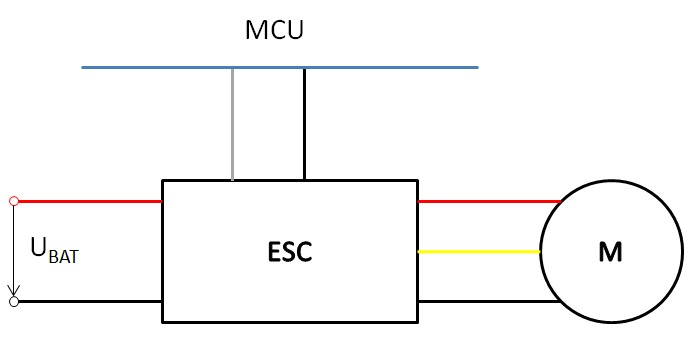
\includegraphics[width=.90\textwidth]{sec4/images/Skizze_BLDC_ESC} 
\centering
\captionsetup{width=.95\textwidth}
\caption[Skizze zur Beschaltung eines \ac{ESC}s und \ac{BLDCMot}s]{Skizze zur Beschaltung eines \ac{ESC}s und \ac{BLDCMot}s; Versorgungsspannung des \ac{ESC}s in rot und schwarz (Masse), \ac{PWM}-Signalleitungen in grau und schwarz (Masse) und Anschlussleitungen des \ac{BLDCMot}s in rot, gelb und schwarz}\centering
\label{fig:SkizzeAntrieb}
\end{figure}

\subsection{Montage der Antriebskomponenten}\label{Sec4Sub2}

Die Komponenten des Fahrzeugantriebs, der über zwei \acp{BLDCMot} realisiert ist, sind auf der unteren Fahrzeugebene montiert. Die Motoren selbst sind mit zwei Schrauben an der Karosserie befestigt. An der Welle der Motoren befindet sich je ein Zahnrad mit 13 Zähnen, welches ein weiteres Zahnrad mit 90 Zähnen antreibt, das an der Antriebswelle befestigt ist. Das heißt, dass sich die Reifen bei 6,923 Umdrehungen der Motorwelle genau einmal drehen.\vspace{11pt}

In Abbildung \ref{fig:MontageMotorUebersetzung} sind die montierten Komponenten des linken Antriebs abgebildet. Die Befestigungsschrauben der Motoren sind dabei in rot hervorgehoben, die Befestigungsschrauben des Zahnrads der Antriebswelle in blau und die Befestigung des Reifens in orange. Das Zahnrad der Motorwelle ist durch Erhitzen geweitet und auf die Welle aufgesetzt worden. Zur Sicherheit dient hier etwas Sekundenkleber dazu, dass sich das Zahnrad auf der Welle nicht durchdreht. Sekundenkleber ist hier völlig ausreichend, da aufgrund der Übersetzung nur 1/7 des auf die Reifen wirkenden Moments auf das Zahnrad der Motorwelle wirkt.

\begin{figure}[H] %H für Positionierung hier
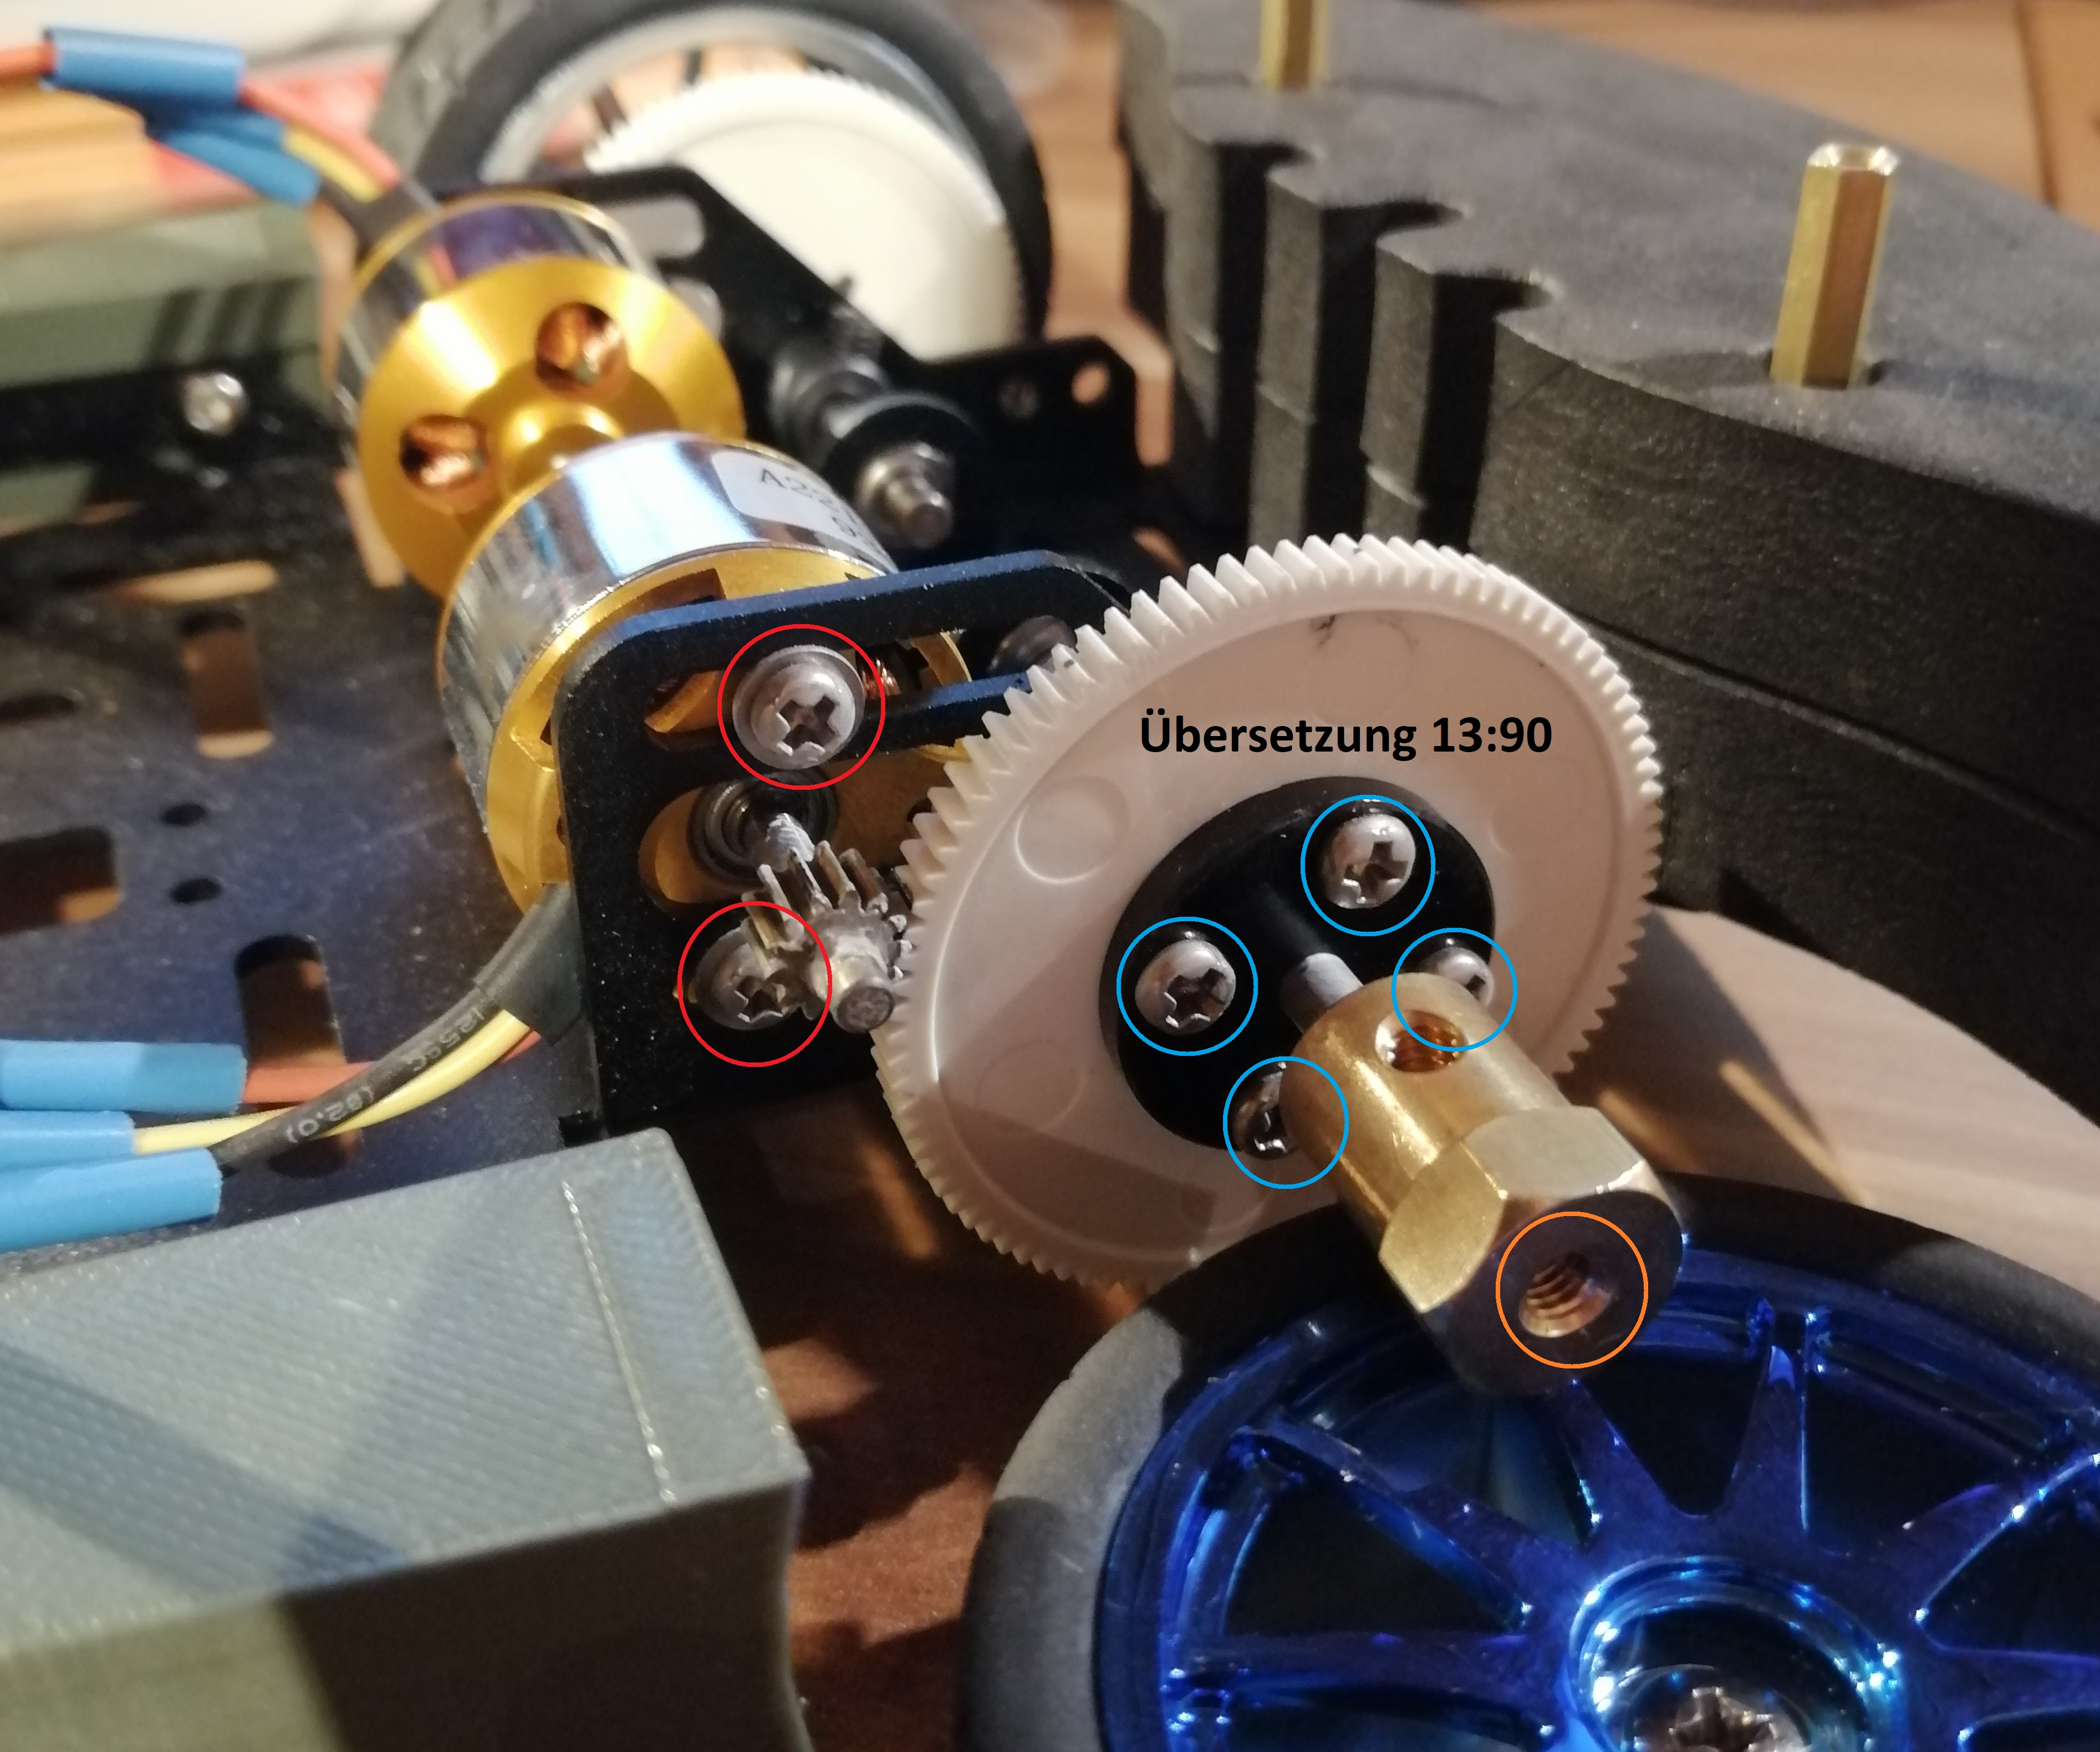
\includegraphics[width=.90\textwidth]{sec4/images/MontageMotorUebersetzung} 
\centering
\captionsetup{width=.95\textwidth}
\caption[Montage der Antriebskomponenten]{Montage der \acp{BLDCMot} und Übersetzung auf die Antriebsachse; In rot die Befestigung des \ac{BLDCMot}s, in blau die Befestigung des Zahnrads an der Antriebswelle und in orange die Befestigung des Reifens}\centering
\label{fig:MontageMotorUebersetzung}
\end{figure}

\subsection{Konfiguration der Motorcontroller}\label{Sec4Sub3}

Die beiden Motorcontroller erwarten nach dem Zuschalten der Spannungsversorgung eine Initialisierungssequenz. Das Power-On-Ereignis wird vom \ac{ESC} mit drei Tönen (tief, mittel, hoch) signalisiert. Im Anschluss daran soll der Wert an der Signalleitung größer als 0\% sein. Das bedeutet, dass ein \ac{PWM}-Signal angelegt werden muss, welches eine Drehzahl N $\geq$ 0rpm repräsentiert. Der \ac{ESC} quittiert das Erkennen des \ac{PWM}-Signals mit einem tiefen Ton. Die Initialisierungssequenz ist allerdings erst dann beendet, wenn das \ac{PWM}-Signal an der Signalleitung zuerst vergrößert und dann auf 0\% verringert wird (N = 0rpm). Dabei gibt der \ac{ESC} einen letzten, hohen Ton von sich. Der Ablauf der Initialisierungssequenz ist in Abbildung \ref{fig:initESC} dargestellt. Nach dem letzten Ton ist die Initialisierung beendet und der \ac{BLDCMot} dreht sich in Abhängigkeit des an der Signalleitung anliegenden \ac{PWM}-Signals. 

\begin{figure}[H] %H für Positionierung hier
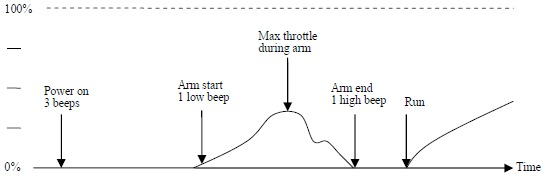
\includegraphics[width=.70\textwidth]{sec4/images/BLDCInit} 
\centering
\captionsetup{width=.95\textwidth}
\caption[Initialisierungssequenz der \ac{ESC}s]{Wert an der Signalleitung für die Initialisierungssequenz über der Zeit; 0\% entspricht dem \ac{PWM}-Tastgrad für den Stillstand und 100\% dem für die maximal erreichbare Drehzahl}\centering
\label{fig:initESC}
\end{figure}

Da die \ac{ESC}s individuell konfiguriert werden können und in der Dokumentation zu wenige Angaben gemacht werden, ist der Tastgrad für die Werte 0\% (Stillstand) und 100\% (maximal erreichbare Drehzahl) unbekannt. Deshalb ist es nicht möglich zu wissen, welche \ac{PWM}-Tastgrade für die Initialisierungssequenz verwendet werden müssen. Über die Konfiguration der \ac{ESC}s können die Grenzen für 0\% und 100\% selbst festgelegt werden. Für das Flashen der Motorcontroller wird die Software \glqq{}BLHeliSuite\grqq{} verwendet. Die Verbindung zwischen den \ac{ESC}s und der Software stellt ein Arduino Nano her.\vspace{11pt}

Der Arduino Nano muss zuvor mit einer neuen Software beschrieben werden. Um die \ac{ESC}s flashen zu können wird der Signalpin des zu programmierenden \ac{ESC} mit dem Pin D3 und der Massepin der Signalleitung mit einem Massepin des Arduino Nano verbunden. Danach wird in der Software \glqq{}BLHeliSuite\grqq{} im Reiter \glqq{}Make Interface\grqq{} eine neue Schnittstelle erstellt (siehe Abbildung \ref{fig:ConfigBLHeliSuite}). Auf der rechten Seite des Programm-Fensters wird ein Arduino Nano als Schnittstelle eingerichtet. Mit einem Klick auf den Button \glqq{}Arduino 4way-interface\grqq{} wird die neue Software, durch die die \ac{ESC}s neu konfiguriert werden können, auf den Arduino Nano geladen.

\begin{figure}[H] %H für Positionierung hier
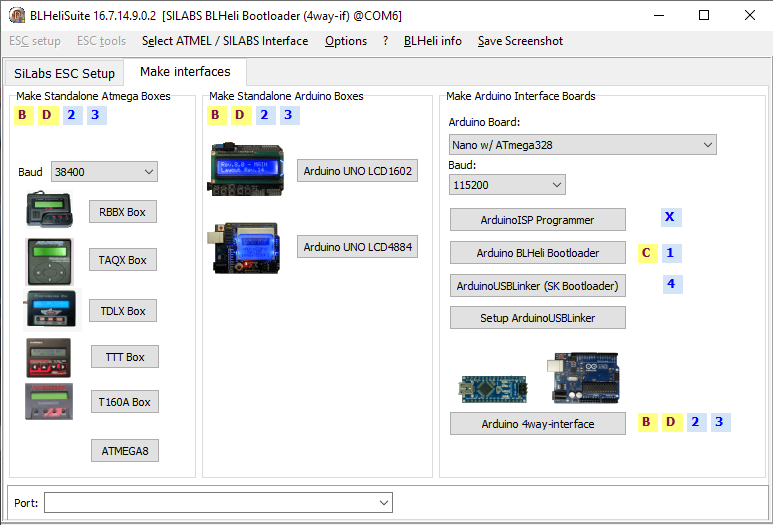
\includegraphics[width=.75\textwidth]{sec4/images/Config_BLHeliSuite} 
\centering
\captionsetup{width=.95\textwidth}
\caption[Programmierung des Arduino Nano zur \ac{ESC}-Konfiguration]{Programmierung des Arduino Nano zur \ac{ESC}-Konfiguration mit der Software BLHeliSuite}\centering
\label{fig:ConfigBLHeliSuite}
\end{figure}

Nach dem Programmieren des Arduino Nano wird die Kommunikation der BLHeliSuite-Software mit dem \ac{ESC} hergestellt. Über die Schaltfläche \glqq{}Read Setup\grqq{} werden die voreingestellten Parameter des \ac{ESC} ausgelesen. Im nächsten Schritt werden die Zeiten für die Werte \glqq{}PPM min Throttle\grqq{} (0\% Aussteuergrad) und \glqq{}PPM max Throttle\grqq{} (100\% Aussteuergrad) auf 1100µs und 1900µs angepasst. Alle vorgenommenen Einstellungen sind in Abbildung \ref{fig:BLHeliSuite} einsehbar. Die Werte werden über die Betätigung der Schaltfläche \glqq{}Write Setup\grqq{} auf den \ac{ESC} geladen. Da jetzt die Werte für 0\% und 100\% Aussteuerung bekannt sind, können die einzelnen Schritte der Initialisierung im Programm des Fahrzeugs abgearbeitet werden.

\begin{figure}[H] %H für Positionierung hier
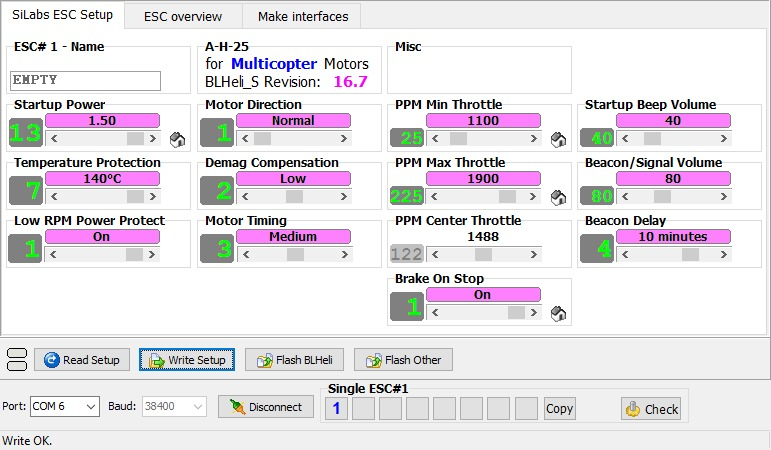
\includegraphics[width=.75\textwidth]{sec4/images/ESC_config} 
\centering
\captionsetup{width=.95\textwidth}
\caption[Parameter der neuen \ac{ESC}-Konfiguration]{Konfiguration der \ac{ESC}s mit der Software \glqq{}BLHeliSuite\grqq{}}\centering
\label{fig:BLHeliSuite}
\end{figure}

\subsection{Programmierung des Antriebsbausteins}\label{Sec4Sub4}

Der Antriebsbaustein der Software ist in zwei Dateien unterteilt, die Dateien \glqq{}drive.c\grqq{} und \glqq{}drive.h\grqq{}. Die Datei \glqq{}drive.h\grqq{} enthält alle relevanten Bibliotheken und Prototypen für die Datei \glqq{}drive.c\grqq{}.\vspace{11pt}

Außer der Einbindung der Bibliotheken und der Prototypen der Funktionen aus der Datei \glqq{}drive.c\grqq{} sind hier auch die Parameter für die Initialisierungssequenz der \ac{ESC}s und für die Initialisierung des Timers für die \ac{PWM}-Signale hinterlegt (Abbildung \ref{fig:DriveH}). 

\begin{figure}[H] %H für Positionierung hier
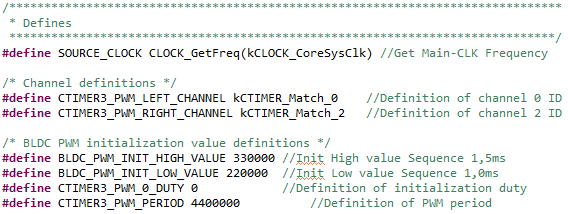
\includegraphics[width=.5\textwidth]{sec4/images/DriveH} 
\centering
\captionsetup{width=.95\textwidth}
\caption[Relevante Zeilen der Datei \glqq{}drive.h\grqq{}]{Relevante Zeilen der Datei \glqq{}drive.h\grqq{} mit den Parametern für die Initialisierungssequenz der \ac{ESC}s und für die Initialisierung des \ac{PWM}-Timers}\centering
\label{fig:DriveH}
\end{figure}

Für die \ac{PWM}-Periodendauer wird bei der Initialisierung ein Wert von 4.400.000 Takten festgesetzt, woraus mit einer \ac{CPU}-Taktfrequenz von 220MHz (220.000.000 Takte pro Sekunde) eine Periodendauer von 20ms resultiert. Die Pulsbreite wird während des Programmablaufs regelmäßig überschrieben.\vspace{11pt}

Der \ac{ESC}-Initialisierungswert für den Stillstand (\glqq{}BLDC\_PWM\_INIT\_LOW\_VALUE\grqq{}, 220.000) entspricht hier einer \ac{PWM}-Pulsbreite von 1,0ms und der Initialisierungswert für die in etwa mittlere Aussteuerung (\glqq{}BLDC\_PWM\_INIT\_HIGH\_VALUE\grqq{}, 330.000) einer Breite von 1,5ms. Die volle Aussteuerung der Motoren wird, wie über die \glqq{}BLHeliSuite\grqq{} festgelegt, bei einer Pulsdauer von 1,9ms erreicht (\glqq{}BLDC\_PWM\_FULLTHROTTLE\grqq{}, 418.000). Eine Drehzahl von N = 0rpm wird theoretisch über die bei der \ac{ESC}-Konfiguration festgelegten 1,1ms ermöglicht (242.000). Da das \ac{PWM}-Signal leicht abweicht, wird ein etwas geringerer Wert veranlagt (\glqq{}BLDC\_PWM\_STOPTHROTTLE\grqq{}, 240.000 = 1,09ms). Damit wird sichergestellt, dass sich die Räder im Stillstand nicht drehen.\vspace{11pt}

Auch die beiden \ac{PWM}-Timer (einer je Motorcontroller) benötigen bei der Initialisierung einige Parameter, deren Werte in der Datei \glqq{}drive.h\grqq{} festgelegt sind (PWM-Periodendauer, \ac{PWM}-Pulsdauer, Channel). Die Channel werden auf das Timer Match Register 2 (rechter Antrieb, \glqq{}kCTIMER\_Match\_2\grqq{}) und auf das Timer Match Register 0 (linker Antrieb, \glqq{}kCTIMER\_Match\_0\grqq{}) festgelegt, was bei dem verwendeten Controller den Pins P0.27 (rechts) und P3.10 (links) entspricht. Der Pin P3.10 wird auf der Controllerplatine über den Pin 7 und der Pin P0.27 über den Pin 12 der Buchsenleiste J13 nach außen geführt. Der Anschluss der Motorcontroller ist über den Anhang \glqq{}\nameref{SecAtt1}\grqq{} nachvollziehbar.


\begin{figure}[H] %H für Positionierung hier
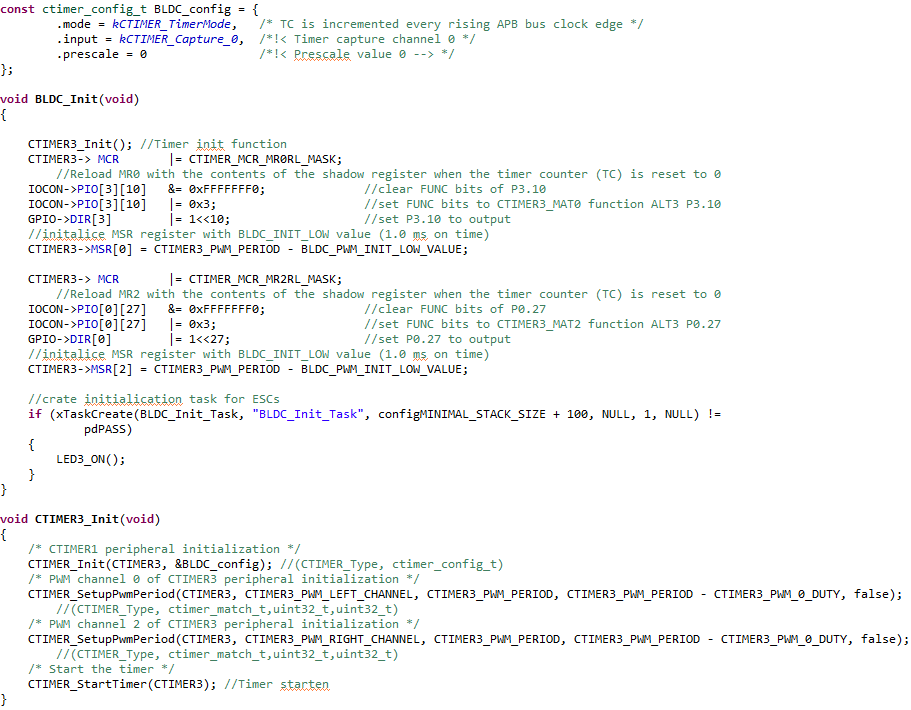
\includegraphics[width=.93\textwidth]{sec4/images/DriveC1} 
\centering
\captionsetup{width=.95\textwidth}
\caption[Funktionen BLDC\_Init und CTIMER3\_Init der Datei \glqq{}drive.c\grqq{}]{Funktionen BLDC\_Init und CTIMER3\_Init der Datei \glqq{}drive.c\grqq{}}\centering
\label{fig:DriveC1}
\end{figure}

Die Datei \glqq{}drive.c\grqq{} enthält die Funktionen zur Initialisierung der für die Verwendung der Antriebe notwendigen Controller-Peripherie (siehe Abbildung \ref{fig:DriveC1}) und zur Initialisierung der Motorcontroller (siehe Abbildung \ref{fig:DriveC2}).\vspace{11pt}

In der Funktion BLDC\_Init wird zuerst die Funktion CTIMER3\_Init aufgerufen, welche die beiden vorher festgelegten Kanäle des Timers C3 (\glqq{}kCTIMER\_Match\_0\grqq{} und \glqq{}kCTIMER\_Match\_2\grqq{}) mit den in der Datei ''drive.h'' festgelegten Parametern als \ac{PWM}-Timer mit einer Periodendauer von 20ms und einer Pulsdauer von 0ms initialisiert. Im Anschluss daran wird einzeln für beide Kanäle festgelegt, dass bei einem Timer-Überlauf die neuen Daten für die Pulslängen aus den Shadow-Registern geladen werden sollen. Zum Ändern der Geschwindigkeit eines der beiden Antriebe muss deshalb lediglich ein neuer Wert in das Shadow-Register geschrieben werden. Hier muss allerdings aufgepasst werden, da das Register nicht die Pulsbreite (On-Time) sondern die Off-Time erwartet. Deshalb muss der Wert, der eingetragen wird, der Periodendauer abzüglich der Pulsdauer entsprechen. Zusätzlich werden in der Funktion BLDC\_Init auch die Pins P3.10 und P0.27 für die Verwendung als \ac{PWM}-Ausgang des Timers C konfiguriert. Am Ende wird noch der erste \ac{ESC}-Initialisierungswert in die beiden Shadow-Register geschrieben, bevor die \ac{ESC}-Initialisierungsfunktion aufgerufen wird (siehe Abbildung \ref{fig:DriveC2}).

\begin{figure}[H] %H für Positionierung hier
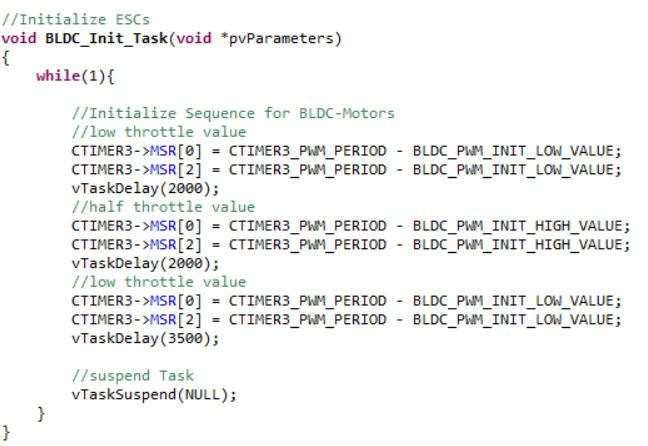
\includegraphics[width=.75\textwidth]{sec4/images/DriveC2} 
\centering
\captionsetup{width=.95\textwidth}
\caption[Funktion BLDC\_Init\_Task der Datei \glqq{}drive.c\grqq{}]{Funktion BLDC\_Init\_Task der Datei \glqq{}drive.c\grqq{} zum Durchlaufen der Initialisierungssequenz der \ac{ESC}s}\centering
\label{fig:DriveC2}
\end{figure}

Der Task BLDC\_Init\_Task beginnt mit dem Befüllen der Shadow-Register mit dem ersten Initialisierungswert. Nach einer Wartezeit von 2s wird der zweite Initialisierungswert in die Register geschrieben. Ebenfalls nach einer Zeit von 2s wird dann wieder der erste Initialisierungswert in die Shadow-Register geschrieben und die Initialisierung der \ac{ESC}s ist abgeschlossen. Die Wartezeiten sind notwendig, damit die \ac{ESC}s Zeit haben, die Änderungen zu erfassen.

\newpage
\subsection{Drehzahlmessung}\label{Sec4Sub5}

\subsubsection{Erörterung der Notwendigkeit einer Drehzahlmessung}\label{Sec4Sub5Sub1}

Die Quellspannung von Akkus verringert sich mit steigender Betriebszeit, weshalb bei vorherigen Fahrzeug-Versionen eine Drehzahlmessung benötigt wird, um über eine Regelung die Spannungsabhängigkeit der Drehzahl bei \acp{DCMot} ausgleichen zu können. Probleme hat diese Abhängigkeit vor allem beim Überfahren eines Hügels bereitet. Da die in den vorangegangenen Fahrzeugmodellen verwendeten \acp{DCMot} durch \acp{BLDCMot} ersetzt wurden, stellt sich allerdings wieder die Frage nach der Notwendigkeit einer Drehzahlmessung. Die Variation der Drehzahl funktioniert bei \acp{DCMot} über die Änderung der Betriebsspannung, was auch die Abhängigkeit von der Versorgungsspannung erklärt. Die Drehzahlvariation bei einem \ac{BLDCMot} wird hingegen über eine Frequenzänderung der Strangspannungen realisiert. Zur Klärung der Frage nach einer Spannungsabhängigkeit der \acp{BLDCMot}, wird eine Messung am Prüfstand durchgeführt.\vspace{11pt}

Für die Durchführung der Messung wird ein bereits vorhandener Prüfstand für Modellfahrzeuge verwendet, welcher im Rahmen einer Bachelor-Abschlussarbeit an der HAW Landshut erstellt wurde. In Abbildung \ref{fig:Pruefstand01} ist der Messaufbau zu sehen. Mithilfe eines Drahtes wird das Heck des Fahrzeugs so an der Grundplatte des Prüfstands befestigt, dass die Reifen einen besseren Halt auf den Rollen des Prüfstands haben. An den Vorderreifen ist das Fahrzeug ebenfalls festgeschnallt. 


\begin{figure}[H] %H für Positionierung hier
\includegraphics[width=.75\textwidth]{sec4/images/Pruefstand_Messung_UAbhängigkeit} 
\centering
\captionsetup{width=.95\textwidth}
\caption[Messaufbau zur Prüfung der Spannungsabhängigkeit der \acp{BLDCMot}]{Messaufbau zur Prüfung der Spannungsabhängigkeit der \acp{BLDCMot}; in blau die Befestigung des Hecks an der Grundplatte des Prüfstands, in gelb die Befestigung der Vorderreifen am Prüfstand, in rot die DC-Motoren zur Spannungsmessung}\centering
\label{fig:Pruefstand01}
\end{figure}

Zur Überprüfung einer eventuellen Drehzahlabhängigkeit der \acp{BLDCMot} von der Versorgungsspannung wird die Spannung an den \acp{DCMot} des Prüfstands gemessen, weil diese direkt proportional zur Drehzahl ist (siehe Gleichung \ref{eq1}). Da die Drehmomentkonstante k\textsubscript{i} bei hohen Drehzahlen leicht einbricht, ist die Abhängigkeit der gemessenen Spannung von der Drehzahl allerdings nur annähernd linear. Aufgrund der für die Messung konstant eingestellten Pulsbreite von 1,5ms, spielt der Einbruch der Drehmomentkonstante allerdings keine große Rolle, da sich die Drehzahl wenn überhaupt nur sehr gering ändert. Dieser Zusammenhang kann deshalb vereinfachend als linear angenommen werden kann. Die Versorgungsspannung der \acp{ESC} wird für die Aufnahme verschiedener Messwerte zwischen 6,1V und 8V variiert. Ändert sich die gemessene Spannung mit der Variation der Versorgungsspannung, so ist das ein hinreichender Beweis dafür, dass die Drehzahl der \acp{BLDCMot} spannungsabhängig ist. Die Ergebnisse der Messreihe aus Tabelle \ref{tab:PrüfstandMess01} sind zur einfacheren Auswertung in Abbildung \ref{fig:Pruefstand02} visualisiert.

\begin{equation}\label{eq1}
U_A = k_i \cdot N \cdot \frac{\pi}{30}
\end{equation}

\begin{table}[H]
\begin{tabular}{|c|c|c|c|c|c|c|c|c|c|c|}
\hline
\rule{0pt}{15pt} Messung & 1&2&3&4&5&6&7&8&9&10 \\
\hline
U\textsubscript{Versorgung} [$V$]&8.0&7.9&7.8&7.7&7.6&7.5&7.4&7.3&7.2&7.1 \\ 
\hline
U\textsubscript{Messung} [$V$]&5.80&5.75&5.65&5.57&5.48&5.40&5.35&5.25&5.18&5.09 \\
\hline
\hline
\rule{0pt}{15pt} Messung & 11&12&13&14&15&16&17&18&19&20 \\
\hline
U\textsubscript{Versorgung} [$V$]&7.0&6.9&6.8&6.7&6.6&6.5&6.4&6.3&6.2&6.1 \\ 
\hline
U\textsubscript{Messung} [$V$]&5.05&4.96&4.87&4.82&4.69&4.73&4.66&4.60&4.50&4.45 \\
\hline
\end{tabular}
\centering
\captionsetup{width=.95\textwidth}
\caption[Messreihe 1: Spannungsabhängigkeit Drehzahl]{Messreihe 1: Messwerte für Überprüfung einer eventuellen Spannungsabhängigkeit der Drehzahl}\centering
\label{tab:PrüfstandMess01}
\end{table}

Aus Abbildung \ref{fig:Pruefstand02} können einige wertvolle Erkenntnisse abgeleitet werden. Zum einen ist die Drehzahl, welche proportional zu der an den \ac{DCMot} gemessenen Ankerspannung U\textsubscript{Messung} ist, nicht konstant. Die Drehzahl der \acp{BLDCMot} ist also von der Versorgungsspannung der \acp{ESC} abhängig, andernfalls wäre die resultierende Gerade eine Horizontale.\vspace{11pt}

Die sich aus der Messreihe ergebenen Erkenntnisse machen eine Drehzahlregelung sinnvoll, da während der Durchfahrt des Parcours nicht die volle Drehzahl benötigt wird und eine Regelung es ermöglicht, die vorgegebene Drehzahl auch bei fortschreitender Entladung des Akkus zu fahren. Wird eine feste Geschwindigkeit vorgegeben, kann die Regelung bei fallender Versorgungsspannung der \acp{ESC} das \ac{PWM}-Signal bis zur Stellgrenze (Pulsbreite = 1,9ms) erhöhen. Erst bei Erreichen der Stellgrenze nimmt die Drehzahl linear mit der Versorgungsspannung ab.\vspace{11pt}


\begin{figure}[H] %H für Positionierung hier
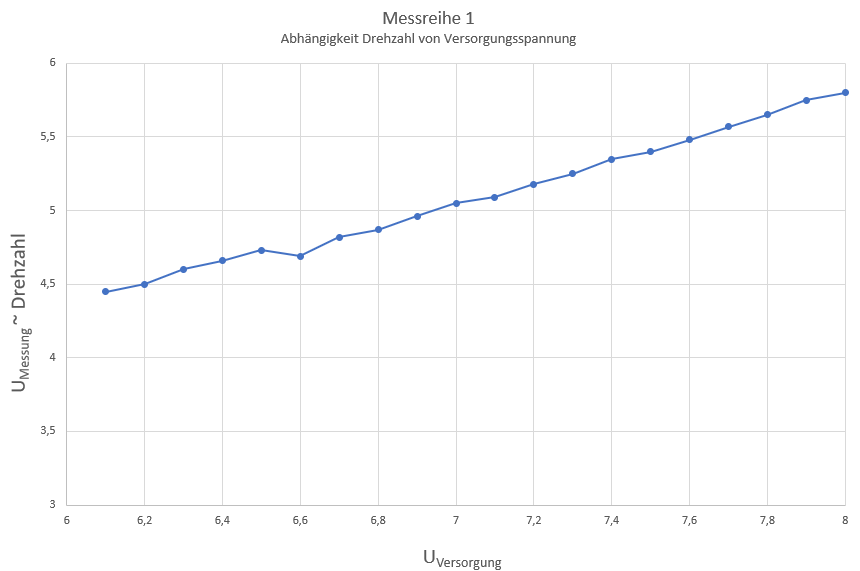
\includegraphics[width=.90\textwidth]{sec4/images/PruefstandMess02} 
\centering
\captionsetup{width=.95\textwidth}
\caption[]{}\centering
\label{fig:Pruefstand02}
\end{figure}


Beim NXP-Cup muss das Fahrzeug nach dem Überfahren der Ziellinie innerhalb von zwei Metern anhalten. In der Konfiguration der \acp{ESC} bietet sich dafür die Einstellung \glqq{}Break On Stop\grqq{} an, mit der das Fahrzeug bei einer PWM-Pulsdauer von 1ms (Stop-Throttle) aktiv bremst, indem die drei Phasen der \acp{BLDCMot} auf Masse geschlossen werden. Die Bremskraft reicht aus, um das Fahrzeug innerhalb von ca. 30cm zum Stehen zu bringen. \vspace{11pt}

***Problem wegdriften bzw. Rutschen der Reifen weil blockiert -> wegrutschen nach rechts Grund evtl unterschiedlich feste Montage der Reifen***\vspace{11pt}

***Für später Probleme wegen 1s Strafzeit, wenn nach der Ziellinie die Strecke verlassen wird oder nicht in 2m angehalten wird***




\subsubsection{Auswahl des Messprinzips}\label{Sec4Sub5Sub2}
***MARKUS***

1.: Hallsensormodul mit zwei um 90° versetzten HallSensoren für Drehzahl und Magentfolie
2.: Tiefpassfilterung und Komparator für Drehzahl

1: - Pro: spricht, dass auch Drehrichtung aufgenommen werden kann und das mit nur einem Bauteil (Hallsensormodul mit zwei um 90°versetzten Hallsensoren)
 - Contra erste spricht, dass Magnetfolie abgehen kann, 
 - Contra dass 3D Druckteil Halterung konstruiert und gedruckt werden muss
 - Kosten?
 - Pro: bringt direkt für GPIO notwendige Signale 

2:  - Pro: Man kann Signal selbst so aufbereiten, wie man es will/braucht
- Kosten?
- BLDC variieren Drehzahl über Frequenz --> Frequenz kann man mit Zähler leicht messen
- eine Phase je BLDC für Drehzahl
- zwei Phasen je BLDC um auch Drehrichtung zu bekommen --> brauchen wir aber nicht, weil wegen ESC nur vorwärts fahren

Warum haben wir uns für 2 entschieden? 


\subsubsection{Hardware für die Drehzahlmessung}\label{Sec4Sub5Sub3}
***MARKUS***

\subsubsection{Programmierung des Drehzahlmessungsbausteins}\label{Sec4Sub5Sub4}
***MARKUS***

\newpage